\documentclass[conference]{IEEEtran}
\IEEEoverridecommandlockouts

\usepackage{cite}
\usepackage{amsmath,amssymb,amsfonts}
\usepackage{graphicx}
\usepackage{textcomp}
\usepackage{xcolor}
\usepackage{booktabs}
\usepackage{multirow}
\usepackage{array}
\usepackage[hyphens]{url}
\usepackage{tikz}
\usetikzlibrary{arrows.meta,positioning,fit,backgrounds,calc}

\def\BibTeX{{\rm B\kern-.05em{\sc i\kern-.025em b}\kern-.08em
    T\kern-.1667em\lower.7ex\hbox{E}\kern-.125emX}}

\newcommand{\miou}{mIoU}

\begin{document}

\title{Making OpenAD Robust to Query Phrasing in 3D Affordance Detection}

\author{\IEEEauthorblockN{Mehreen Hossain Chowdhury}
\IEEEauthorblockA{\textit{Dept.\ of CSE} \\
\textit{Islamic University of Technology}\\
Gazipur, Bangladesh \\
ID 210041219}
\and
\IEEEauthorblockN{Sumaiya Ahmed Rani}
\IEEEauthorblockA{\textit{Dept.\ of CSE} \\
\textit{Islamic University of Technology}\\
Gazipur, Bangladesh \\
ID 210041223}
\and
\IEEEauthorblockN{Jannatul Fardus Rakhi}
\IEEEauthorblockA{\textit{Dept.\ of CSE} \\
\textit{Islamic University of Technology}\\
Gazipur, Bangladesh \\
ID 210041237}
}

\maketitle

\begin{abstract}
Open-vocabulary affordance detection allows a robot or assistive system to locate the part of a 3D object associated with a free-form language query. OpenAD does this by comparing PointNet++ features at each point with CLIP text embeddings. However, the model is trained on single-word labels, while users are more likely to ask questions such as ``Where can I grasp this object?'' This work examines how well OpenAD handles that difference in wording. We first reproduce the released model on the 3D AffordanceNet validation split, obtaining 14.40 mIoU compared with the reported 14.37. Rephrasing five affordances as questions or descriptions reduces full-vocabulary mIoU from about 41 to about 30, although the resulting score maps remain spatially correlated. To improve this behaviour, we fine-tune the model with randomly sampled paraphrases while leaving the architecture, CLIP encoder, and point labels unchanged. Updating 101,377 parameters (less than six percent of the point network) improves mIoU on held-out questions by 11.2 points and on held-out descriptions by 10.5 points. This recovers more than 90 percent of the loss caused by rephrasing without reducing performance on the original labels. Experiments with three unfreezing depths show that the alignment head alone provides most of the gain. On OpenAD's synonym benchmark, mIoU increases from 14.40 to 18.66; nearly all of this improvement comes from the five affordances used during fine-tuning, while the other 13 remain stable. Qualitative examples and an interactive prototype further show how the model responds to different phrasings. Overall, a small amount of prompt-augmented fine-tuning makes OpenAD considerably less sensitive to wording.
\end{abstract}

\begin{IEEEkeywords}
affordance detection, open vocabulary, point clouds, CLIP, prompt robustness, fine-tuning
\end{IEEEkeywords}

%% ------------------------------------------------------------------
\section{Introduction}
\label{sec:intro}

An affordance describes what an object allows an agent to do. A mug can be grasped by its handle, a chair can be sat on, and a knife cuts with its blade~\cite{gibson1979}. For a robot or assistive system, knowing \emph{where} an action can be performed is often more useful than simply recognising the object. Per-point affordance detection addresses this need by assigning an affordance label to each point in a 3D point cloud~\cite{affordancenet}. Most earlier methods use a fixed set of classes, so adding a new action requires new annotations and retraining the classifier.

OpenAD~\cite{openad} replaces this fixed classifier with a shared point--text embedding space. A frozen CLIP encoder~\cite{clip} embeds the text queries, and each point is assigned to the nearest query in that space. This makes it possible, at least in principle, to use new words at test time. Yet people rarely reproduce the exact labels used during training. Where the model saw only ``grasp'', a user might ask ``Where can I grasp this object?'' or describe ``the part used for holding''. A practical natural-language interface therefore depends on whether the detector can recognise the same intent across these different forms.

We investigate this issue using the released OpenAD PointNet++ model and the 3D AffordanceNet dataset. The experiments address five questions:
\begin{enumerate}
\item Can we reproduce the published closed-set and open-vocabulary numbers with the released checkpoint and our own evaluation code?
\item How much does accuracy change when the training words of some affordances are replaced by questions or descriptions with the same meaning?
\item Can a lightweight adaptation that changes only the language supervision restore accuracy, without touching the point backbone, the text encoder or the ground-truth masks?
\item Does the restored accuracy transfer to phrasings that were never used for training?
\item How many parameters need to change, and where in the network does the improvement reside?
\end{enumerate}

The work makes five main contributions. First, we build an evaluation harness for arbitrary query strings and validate it against the official evaluator and hand-checked unit tests. Second, we measure the effect of phrasing at both the class and score-map levels. Third, we introduce prompt-augmented fine-tuning for the alignment head and final feature-propagation layer (101,377 parameters) and evaluate it on phrases fixed before training. Fourth, we compare three unfreezing depths, from 67,073 to 743,041 trainable parameters. Finally, we examine representative successes and failures and provide an interactive prototype based on the same model.

The main result is straightforward: natural rephrasings of five affordances reduce the released model's score by about 12 mIoU points, and fine-tuning 101,377 parameters with paraphrase supervision recovers more than 90 percent of this loss on unseen wordings. Training over seven times as many parameters offers no meaningful additional benefit, suggesting that most of the problem lies in the final point-to-text alignment.

All experiments start from the weights released by the OpenAD authors. We keep the architecture, CLIP text encoder, per-point labels, and loss unchanged; only the language supervision differs. The aim is not to propose a new architecture, but to measure a practical weakness and test a lightweight remedy. Throughout the report, ``cited'' denotes results taken from the OpenAD paper, while ``ours'' denotes results produced by our repository\footnote{\url{https://github.com/mehreen019/Open-Vocabulary-3D-Affordance-Detection}}.

%% ------------------------------------------------------------------
\section{Related Work}
\label{sec:related}

\textbf{Affordance detection in 3D.} 3D AffordanceNet~\cite{affordancenet} provides a benchmark of point clouds with per-point affordance labels and evaluates closed-set networks in full-shape and partial-view settings. Other work predicts affordance heat maps from object-object interaction~\cite{o2oafford}, from 2D interaction images~\cite{iagnet}, or from natural-language queries~\cite{laso}. OpenAD~\cite{openad} introduced the open-vocabulary version of the task on point clouds by learning a shared space for point features and text. Follow-up work adds knowledge distillation and a text-point correlation module to this setting~\cite{vo2024}; here we study instead how the released OpenAD model responds to the wording of the query.

\textbf{Language-driven point cloud understanding.} CLIP~\cite{clip} aligns images and text at web scale. PointCLIP~\cite{pointclip} projects point clouds to depth images to reuse CLIP for classification, and OpenScene~\cite{openscene} distils CLIP features into a 3D network for open-vocabulary scene understanding. OpenAD differs in that its point network is trained directly against frozen CLIP text embeddings, so no image branch is needed.

\textbf{Point networks.} PointNet~\cite{pointnet} processes unordered points with shared per-point MLPs and a symmetric pooling function. PointNet++~\cite{pointnet2} adds a hierarchy of local neighbourhoods obtained by farthest point sampling and ball queries, and dynamic graph convolution~\cite{dgcnn} is an alternative that OpenAD also supports. We use the PointNet++ variant.

\textbf{Prompt sensitivity and adaptation.} It is known that the wording of a text prompt changes the behaviour of CLIP-based classifiers. The original CLIP work uses hand-designed templates and prompt ensembles~\cite{clip}, and CoOp~\cite{coop} learns continuous prompt vectors. Our approach differs in that we keep the text encoder and the text fixed, and instead expose the point-side alignment head to many paraphrases during training. Updating few parameters follows the observation that full fine-tuning can distort pretrained features~\cite{kumar2022}, and is in the spirit of lightweight adaptation of CLIP through feature adapters~\cite{clipadapter} and of robust fine-tuning of zero-shot models~\cite{wortsman2022}.

%% ------------------------------------------------------------------
\section{Dataset and Evaluation Protocol}
\label{sec:data}

\subsection{Dataset}
We use the full-shape setting of 3D AffordanceNet~\cite{affordancenet} as distributed with OpenAD. According to the OpenAD paper~\cite{openad}, the dataset contains 22,949 object instances from 23 object categories and 18 affordance classes. Each object is a point cloud of $N=2048$ points, as fixed in the OpenAD paper, and each point carries one integer label in the released files, either one of 18 affordances or a background class \texttt{none}, giving $19$ classes in total. The affordance names, in label order, are grasp, contain, lift, openable, layable, sittable, support, wrap\_grasp, pourable, move, display, pushable, pull, listen, wear, press, cut, stab and none. We rely on this order matching the dataset labels, which we verified on the data.

The released data provide training and validation splits but no separate test split. Following the OpenAD code, we report results on the 2,285-object validation split. Its categories are highly imbalanced: Table (799 objects) and Chair (611) together make up 62\% of the split, while Scissors, Bag, Keyboard, and Dishwasher contain only 6, 12, 15, and 16 objects, respectively.

\subsection{Preprocessing}
Points are centred on their centroid and divided by the largest distance to the centroid, so that each object lies in the unit sphere. This is the normalisation of the released data loader, and our inference code repeats it for arbitrary input clouds. We apply no geometric augmentation. The only augmentation in this work acts on the language side (Section~\ref{sec:finetune}).

\subsection{Label protocol and open-vocabulary test}
Let $\mathcal{Q}=(q_1,\dots,q_K)$ be a list of query strings aligned with the class indices. In closed-set evaluation, $\mathcal{Q}$ contains the 19 training words. OpenAD tests open-vocabulary behaviour by replacing the 18 affordance words with synonyms while keeping the labels unchanged. The synonyms are grab, accommodate, raise, unlock, rest, take a seat, bear, wrap, pour, reposition, demonstrate, push, drag, hear, clothe, thumb, slice and jab. The class \texttt{none} is kept. The released configuration evaluates these 19 queries, and our close reproduction of the paper's result (Section~\ref{sec:repro}) provides an additional check that we are using the intended benchmark.

\subsection{Metrics}
The predicted class of point $i$ is the index of the query with the highest score, $\hat{y}_i=\arg\max_k S_{ik}$ (Section~\ref{sec:method}). Intersection, union and support are accumulated over all points of all objects in the split. For class $c$, with the bracket equal to 1 if the condition holds and 0 otherwise,
\begin{equation}
\mathrm{IoU}_c=\frac{\sum_i [\hat y_i=c\wedge y_i=c]}{\sum_i [\hat y_i=c\vee y_i=c]+\epsilon},\qquad \epsilon=10^{-6},
\label{eq:iou}
\end{equation}
and $\mathrm{mIoU}=\frac{1}{19}\sum_c \mathrm{IoU}_c$, which includes the background class. We also report point accuracy and mean class accuracy (mean per-class recall). These definitions follow the official evaluator, which we compared line by line with \texttt{utils/eval.py} of the OpenAD repository, and our implementation is tested against hand-computed confusion matrices. All IoU and mIoU values in this report are given in percent, i.e.\ 100 times the quantities of Eq.~\eqref{eq:iou}.

\subsection{Phrasing conditions}
\label{sec:conditions}
A phrasing condition changes only the strings in $\mathcal{Q}$. We studied five affordances, namely grasp, contain, sittable, pourable and cut. For each we wrote phrases in three forms, namely a \emph{label} (a single word), a \emph{question}, and a \emph{description}. The phrases are split into two disjoint groups, \emph{fine-tuning} phrases (7 per affordance, 35 in total) and \emph{held-out} phrases (4 per affordance, 20 in total). The split was written into a version-controlled configuration file before any fine-tuning was run, and a unit test fails if a string occurs in both groups. In a condition such as ``question, held-out'', the five studied affordances are replaced by their held-out question and the other 14 classes keep their canonical word. The labels of the points do not change. Table~\ref{tab:prompts} lists the phrases used for evaluation. The held-out label forms are defined in the configuration but are not part of the comparison of Table~\ref{tab:main}. Four of them (grab, accommodate, take a seat and slice) coincide with OpenAD's synonym queries and are scored in Section~\ref{sec:ov}.

The held-out phrases are new wordings of known affordances, not new affordance concepts. The experiment therefore measures generalisation across phrasing rather than across classes.

\begin{table*}[t]
\caption{Query strings used in the evaluation for the five studied affordances. ``Seen'' phrases are members of the fine-tuning set and ``held-out'' phrases were never used for training or for choosing an epoch. The remaining 14 classes always use their canonical word.}
\label{tab:prompts}
\centering
\small
\newcolumntype{L}[1]{>{\raggedright\arraybackslash}p{#1}}
\begin{tabular}{@{}L{0.08\textwidth}L{0.075\textwidth}L{0.185\textwidth}L{0.185\textwidth}L{0.17\textwidth}L{0.185\textwidth}@{}}
\toprule
Affordance & Canonical & Question, seen & Question, held-out & Description, seen & Description, held-out \\
\midrule
grasp    & grasp    & Where can I grasp this object?      & Where should I take hold of this?         & the part used for holding        & the surface meant for gripping by hand \\
contain  & contain  & Where can this object contain something? & Where does it keep things inside?   & the hollow region that holds contents & the cavity that carries material inside \\
sittable & sittable & Where can I sit on this object?     & Where would a person sit down here?       & the surface you sit on           & the part that supports a seated person \\
pourable & pourable & Where can I pour from this object?  & Where does the liquid come out when tipped? & the opening liquid is poured from & the lip through which contents flow out \\
cut      & cut      & Where can I cut with this object?   & Where is the part that cuts things?       & the sharp edge used to cut       & the honed edge intended for slicing \\
\bottomrule
\end{tabular}
\end{table*}

\subsection{Evaluation noise}
\label{sec:noise}
Farthest point sampling begins from a random point, so repeated evaluations of the same checkpoint vary slightly. We measured this variation before comparing models. Five runs with canonical words produced 41.19, 41.25, 41.28, 41.44, and 41.53 mIoU (mean 41.34; range 0.34). Four runs with held-out questions ranged from 29.22 to 29.63, while held-out descriptions ranged from 30.22 to 30.40. We therefore treat differences below roughly 0.5 mIoU as practically equivalent. Each value in the following tables comes from one evaluation pass; the pretrained rows in Tables~\ref{tab:sens}, \ref{tab:main}, and \ref{tab:ablation} belong to their respective comparison runs.

%% ------------------------------------------------------------------
\section{Method}
\label{sec:method}

\subsection{Task formulation}
The input is a point cloud $P\in\mathbb{R}^{N\times 3}$ and a list of $K$ query strings $\mathcal{Q}$. The output is a matrix $S\in[0,1]^{N\times K}$ whose row $i$ is a probability distribution over the queries for point $i$. Two uses occur in this work. For evaluation, $\mathcal{Q}$ holds all 19 class strings and the prediction is the arg-max. For a single user query, $\mathcal{Q}=(q,\texttt{none})$ and the score of the query, $S_{i1}$, is used as a heat map. Because of the softmax, a score is always relative to the competing queries. The same phrase can receive different scores depending on the other strings in $\mathcal{Q}$, which matters for interpreting the maps in Section~\ref{sec:qual}.

\subsection{Architecture}
Figure~\ref{fig:arch} shows the unchanged OpenAD model, which has three main parts.

\textbf{Point encoder.} A PointNet++ network~\cite{pointnet2} with multi-scale grouping. Set-abstraction layer 1 samples 512 centroids by farthest point sampling and gathers neighbours in balls of radius 0.1, 0.2 and 0.4 (32, 64 and 128 neighbours), applying a shared MLP per scale. Layer 2 samples 128 centroids with radii 0.4 and 0.8 (64 and 128 neighbours), and layer 3 pools all points into one global feature of 1024 dimensions. Three feature-propagation layers then upsample back to $N$ points by inverse-distance interpolation over the three nearest neighbours, concatenated with skip connections, and produce a 128-dimensional feature per point. A $1\times1$ convolution from 128 to 512 channels followed by batch normalisation (the \emph{alignment head}) gives the point embedding $f_i\in\mathbb{R}^{512}$. Without the frozen text encoder, the point network has 1,782,765 parameters, which we counted by instantiating the model.

\textbf{Text encoder.} The ViT-B/32 text transformer of CLIP~\cite{clip}, frozen, maps each query string to $t_k\in\mathbb{R}^{512}$. Its parameters are excluded from every optimiser and its outputs are computed without gradients.

\textbf{Alignment.} Point and text embeddings are compared by cosine similarity, scaled by a learnable scalar $s$ and normalised over the queries,
\begin{equation}
z_{ik}=s\,\frac{f_i^{\top}t_k}{\lVert f_i\rVert\,\lVert t_k\rVert},\qquad S_{ik}=\frac{\exp(z_{ik})}{\sum_{j=1}^{K}\exp(z_{ij})}.
\label{eq:align}
\end{equation}
In the released code $s$ is initialised to $\ln(1/0.07)\approx2.659$ and is used directly, not exponentiated as in CLIP, so the initial temperature is about $0.38$. Reading the released checkpoint shows that training has increased $s$ to 25.41, an effective temperature of about 0.039. Fine-tuning moves it to 25.67.

\begin{figure*}[t]
\centering
\resizebox{\textwidth}{!}{%
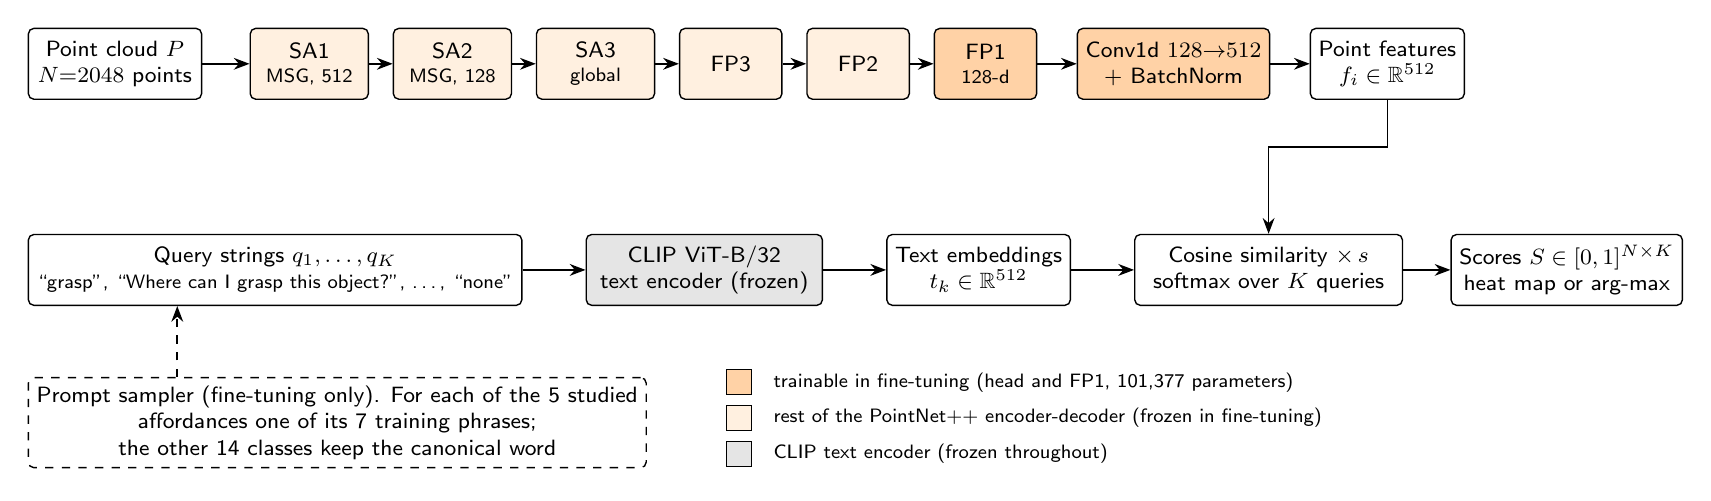
\begin{tikzpicture}[
  font=\sffamily\footnotesize,
  box/.style={draw, rounded corners=2pt, minimum height=9mm, align=center, inner sep=3pt, line width=0.5pt},
  data/.style={box, fill=white},
  frozen/.style={box, fill=black!10},
  backbone/.style={box, fill=orange!12},
  train/.style={box, fill=orange!35},
  arr/.style={-{Stealth[length=2mm]}, line width=0.6pt}
]
% --- point branch
\node[data, minimum width=22mm] (pc) {Point cloud $P$\\$N{=}2048$ points};
\node[backbone, right=6mm of pc, minimum width=15mm] (sa1) {SA1\\[-1pt]{\scriptsize MSG, 512}};
\node[backbone, right=3mm of sa1, minimum width=15mm] (sa2) {SA2\\[-1pt]{\scriptsize MSG, 128}};
\node[backbone, right=3mm of sa2, minimum width=15mm] (sa3) {SA3\\[-1pt]{\scriptsize global}};
\node[backbone, right=3mm of sa3, minimum width=13mm] (fp3) {FP3};
\node[backbone, right=3mm of fp3, minimum width=13mm] (fp2) {FP2};
\node[train, right=3mm of fp2, minimum width=13mm] (fp1) {FP1\\[-1pt]{\scriptsize 128-d}};
\node[train, right=5mm of fp1, minimum width=23mm] (head) {Conv1d $128{\to}512$\\+ BatchNorm};
\node[data, right=5mm of head, minimum width=17mm] (f) {Point features\\$f_i\in\mathbb{R}^{512}$};
\foreach \a/\b in {pc/sa1,sa1/sa2,sa2/sa3,sa3/fp3,fp3/fp2,fp2/fp1,fp1/head,head/f}
  \draw[arr] (\a) -- (\b);

% --- text branch and alignment (second row)
\node[data, minimum width=38mm, anchor=north west] (q) at ([yshift=-17mm]pc.south west)
  {Query strings $q_1,\dots,q_K$\\{\scriptsize ``grasp'', ``Where can I grasp this object?'', \dots, ``none''}};
\node[frozen, right=8mm of q, minimum width=30mm] (clip) {CLIP ViT-B/32\\text encoder (frozen)};
\node[data, right=8mm of clip, minimum width=22mm] (t) {Text embeddings\\$t_k\in\mathbb{R}^{512}$};
\node[box, fill=white, right=8mm of t, minimum width=34mm] (align) {Cosine similarity $\times\,s$\\softmax over $K$ queries};
\node[data, right=6mm of align, minimum width=28mm] (S) {Scores $S\in[0,1]^{N\times K}$\\heat map or arg-max};
\draw[arr] (q) -- (clip);
\draw[arr] (clip) -- (t);
\draw[arr] (t) -- (align);
\draw[arr] (align) -- (S);
\draw[arr] (f.south) -- ++(0,-6mm) -| (align.north);

% --- prompt sampler (fine-tuning only)
\node[box, dashed, minimum width=74mm, anchor=north west] (samp) at ([yshift=-9mm]q.south west)
  {Prompt sampler (fine-tuning only). For each of the 5 studied\\affordances one of its 7 training phrases;\\the other 14 classes keep the canonical word};
\draw[arr, dashed] ([xshift=19mm]samp.north west) -- ([xshift=19mm]q.south west);

% --- legend
\node[draw, fill=orange!35, minimum size=3.2mm, inner sep=0, anchor=north west] (l1) at ([xshift=10mm,yshift=1mm]samp.north east) {};
\node[right=1.5mm of l1, font=\sffamily\scriptsize] {trainable in fine-tuning (head and FP1, 101,377 parameters)};
\node[draw, fill=orange!12, minimum size=3.2mm, inner sep=0, below=1.2mm of l1] (l2) {};
\node[right=1.5mm of l2, font=\sffamily\scriptsize] {rest of the PointNet++ encoder-decoder (frozen in fine-tuning)};
\node[draw, fill=black!10, minimum size=3.2mm, inner sep=0, below=1.2mm of l2] (l3) {};
\node[right=1.5mm of l3, font=\sffamily\scriptsize] {CLIP text encoder (frozen throughout)};
\end{tikzpicture}}
\caption{Pipeline of OpenAD and of our prompt-augmented fine-tuning. Per-point features from a PointNet++ encoder-decoder are compared with CLIP embeddings of arbitrary query strings by cosine similarity, and a softmax over the queries gives per-point scores. The number of queries $K$ is not fixed by the architecture. In fine-tuning only the alignment head is trained, and only the query strings change from step to step; the per-point labels are the same as in the original training.}
\label{fig:arch}
\end{figure*}

\subsection{Objective and original training recipe}
Training uses a class-weighted negative log-likelihood of the softmax output,
\begin{equation}
\mathcal{L}=-\sum_{i=1}^{N} w_{y_i}\log S_{i,y_i},\qquad w_j=\left(\frac{\max_c n_c}{n_j}\right)^{1/3},
\label{eq:loss}
\end{equation}
where $n_j$ is the number of training points of class $j$~\cite{openad}. The weights compensate for the dominance of the background and of frequent affordances. The cube root softens the correction, because full inverse-frequency weights would give very rare classes a large gradient from few points. The released configuration trains for 200 epochs with Adam~\cite{adam} at learning rate $10^{-3}$, weight decay $10^{-4}$, batch size 16, a step decay of the learning rate by a factor 0.5 every 20 epochs (floor $10^{-5}$), and a matching decay of the batch-normalisation momentum~\cite{batchnorm}. We did not repeat this training; the released checkpoint is the starting point of everything below.

\subsection{Why phrasing can matter}
During training, the alignment head sees only 19 distinct text strings. A full sentence and a single word need not occupy the same region of CLIP's embedding space, even when they express the same affordance. A point feature aligned with ``grasp'', for example, may not align equally well with ``Where can I grasp this object?'' In the 19-way prediction, that rephrased query must also compete with 14 classes that still use their original training words. We use this as a working explanation for the sensitivity examined in Section~\ref{sec:results}.

\subsection{Prompt-augmented fine-tuning}
\label{sec:finetune}
Fine-tuning changes only the language supervision. At every training step, we create a query list $\tilde{\mathcal{Q}}$ by sampling one of seven training phrases for each studied affordance (three labels, two questions, and two descriptions). The other classes retain their canonical words, and the same list is used for the whole mini-batch. The point labels, data, loss in Eq.~\eqref{eq:loss}, and class weights remain unchanged. In effect, the head learns to associate an affordance with a family of paraphrases instead of a single word. Held-out phrases are never sampled, and a unit test verifies that the two sets do not overlap.

\textbf{What is trained.} The text side is frozen, so the part of the network that can adapt to new wording lies at the end of the point branch. We therefore study a ladder of three nested configurations, each of which releases more of the decoder. (H) The alignment head (\texttt{conv1}, the affine parameters of \texttt{bn1} and the scale $s$), which is $65{,}536+512+512+512+1=67{,}073$ parameters. (H+F) The head and the last feature-propagation layer \texttt{fp1} (two $1\times1$ convolutions and two batch-normalisation affine pairs, $34{,}304$ parameters), together $101{,}377$ parameters, or 5.7\% of the 1,782,765 parameters of the point network. (D) The head and all three feature-propagation layers \texttt{fp1} to \texttt{fp3}, together $743{,}041$ parameters, or 41.7\%. A tensor-by-tensor comparison with the pretrained checkpoint confirms that exactly 5, 13 and 29 tensors differ in the three configurations (67,073, 101,377 and 743,041 elements) and that the batch-normalisation running statistics are unchanged. The set-abstraction encoder is frozen in all three, and the whole network is kept in evaluation mode so that batch-normalisation statistics do not drift. Confining the update to the end of the network has three motivations. First, the text side is frozen and unchanged, so the discrepancy that we want to remove lies in how point features are mapped into the text space, which is determined by the head and by the layers that produce its input. Second, a small update limits the risk of distorting features that the network learned in 200 epochs~\cite{kumar2022}. Third, it is cheap, since each epoch, including a full validation pass, took about 14 minutes on a laptop GPU.

\textbf{Reported model.} The three configurations are trained with the same data, phrases, loss, learning rate and seed and evaluated on the same conditions, so that differences between them are attributable to capacity alone (Section~\ref{sec:ablation}). We report head plus \texttt{fp1} as the main model because it reached the highest held-out scores of the ladder. As this choice used the held-out scores, its gains are best read together with those of the other two configurations, which lead to the same conclusions.

\textbf{Optimisation.} Adam with learning rate $10^{-4}$ (ten times below the original), no schedule, weight decay $10^{-4}$, batch size 16 with shuffling, seed 1, and 8 epochs (5 epochs for the head-only configuration). These values were fixed in advance and not tuned. The lower rate is meant to adapt the network without undoing pretraining. After every epoch we compute the canonical-word mIoU on the validation split and keep the checkpoint with the highest value. This epoch selection uses canonical words only, so held-out phrasings play no role in choosing the checkpoint within a configuration. The selected checkpoint is that of epoch 4 in all three configurations.

\textbf{Scope.} Five of the 18 affordances are rephrased during training. The other classes see only their canonical word, so they act as the fixed competition against which the rephrased classes are evaluated.

\subsection{Design decisions in brief}
Table~\ref{tab:design} summarises the main design choices and their alternatives. The first five come from OpenAD; the final four are specific to our fine-tuning setup. Section~\ref{sec:ablation} tests the choice of trainable layers empirically.

\begin{table}[t]
\caption{Design decisions, the alternative that each excludes, and the reason.}
\label{tab:design}
\centering
\footnotesize
\newcolumntype{L}[1]{>{\raggedright\arraybackslash}p{#1}}
\begin{tabular}{@{}L{0.25\columnwidth}L{0.22\columnwidth}L{0.40\columnwidth}@{}}
\toprule
Decision & Alternative & Reason \\
\midrule
Frozen CLIP text encoder & Trainable text tower & Keeps the embedding geometry that relates synonyms; training sees only 19 strings, which a trainable encoder could fit without generalising \\
Cosine similarity with a learnable scale & Linear classifier & The number of classes is not fixed, and the scale sharpens a softmax that cosine values in $[-1,1]$ would leave flat \\
Weighted NLL, cube-root weights & Unweighted cross-entropy & Background and frequent affordances dominate the point counts; the cube root limits the gradient of rare classes \\
FPS with multi-scale ball queries & Random sampling, single radius & Even coverage of the surface and robustness to non-uniform density \\
Adam, step-decayed rate & SGD & Published recipe of the released checkpoint, kept as is \\
Vocabulary of fixed length $K{=}19$ during fine-tuning & Paraphrases as extra classes & The softmax, the competition between classes and the metric stay exactly those of pretraining \\
Head and last propagation layer only & Full fine-tuning & The mismatch lies in the point-to-text mapping; few parameters limit forgetting and cost; a ladder of three configurations shows that the gain is already present with the head alone and stays at the same level when the whole decoder is released (Sec.~\ref{sec:ablation}) \\
Learning rate $10^{-4}$ & Original $10^{-3}$ & Adapt the network without undoing pretraining \\
Epoch selection on canonical validation mIoU & Selection on held-out phrasings & Keeps held-out phrasings out of the choice of epoch; the choice among the three layer configurations used them, and all three are reported (Sec.~\ref{sec:ablation}) \\
\bottomrule
\end{tabular}
\end{table}

%% ------------------------------------------------------------------
\section{Experimental Setup and Baselines}
\label{sec:setup}

\textbf{Experimental design.} We begin by reproducing the published result to validate the evaluation harness (Section~\ref{sec:repro}). We then measure sensitivity to wording and compare score maps across phrasings. Prompt-augmented fine-tuning is evaluated on held-out phrases, followed by a capacity study that varies the number of trainable layers (Section~\ref{sec:ablation}). Two query-independent baselines provide context for the metric, while the qualitative analysis and prototype show what the changes look like on individual objects (Section~\ref{sec:qual}).

\textbf{Models compared.} (B0) Two query-independent floors: a majority predictor that assigns every point to the most frequent class (\texttt{none}), and a predictor that draws a uniform random class for every point. Neither sees the point cloud or the query, and both anchor the scale of the metric. (B1) The pretrained OpenAD PointNet++ checkpoint for the full-shape setting released by the authors, loaded without change and pinned to the upstream commit \texttt{b082265}. (B2) Our prompt-augmented fine-tune of B1 that trains the alignment head and the last feature-propagation layer, which is the reported model. (B2$'$, B2$''$) The same fine-tune with the head only and with the whole feature-propagation decoder, which form the capacity ladder together with B2. In the reproduction table we also quote published open-vocabulary baselines (TZSLPC, 3DGenZ and ZSLPC, all with CLIP text encoders) from the OpenAD paper. They are marked as cited.

\textbf{Fairness of the comparison.} The pretrained and the fine-tuned model are evaluated in one script call, on the same validation objects, in the same order, with the same normalisation, the same metric implementation, the same arg-max decision rule and the same query lists. The only quantity that varies between conditions is the set of strings. The fine-tuning phrases, the held-out phrases and the vocabulary order are read from the same configuration files by both the training and the evaluation code. The training loop uses only the official training split. We trained three configurations (seed 1) and report all of them (Section~\ref{sec:ablation}). The learning rate and the number of epochs were fixed in advance and not searched.

\textbf{Implementation.} PyTorch 2.5.1 with CUDA 12.1, Python 3.9.8, OpenAI CLIP package, one NVIDIA RTX 4060 Laptop GPU. The reported fine-tuning took 6,834 s for 8 epochs (about 114 minutes), the head-only configuration 4,261 s for 5 epochs (about 71 minutes) and the decoder configuration 6,726 s for 8 epochs (about 112 minutes), each epoch including a full validation pass. The code contains 16 unit tests that run without a GPU and cover the metrics, the prompt sets and their leakage rules, the freezing logic and the application backend.

%% ------------------------------------------------------------------
\section{Results and Analysis}
\label{sec:results}

\subsection{Reproduction of the pretrained model}
\label{sec:repro}
Table~\ref{tab:repro} compares our evaluation of the released checkpoint with the results reported by OpenAD. In the open-vocabulary setting, we obtain 14.40 mIoU, 46.33\% point accuracy, and 19.63\% mean class accuracy, compared with the published values of 14.37, 46.31, and 19.51. The closed-set mIoU is 41.25 rather than 42.00, and point accuracy is 68.51\% rather than 69.03\%. These small differences indicate that the checkpoint and evaluation pipeline reproduce the original setup closely enough for the later comparisons.

The simple baselines help interpret the scale of these scores. Predicting \texttt{none} for every point yields 43.04\% point accuracy but only 2.27 mIoU, since all 18 affordance classes receive zero IoU. Uniform random prediction gives 1.47 mIoU and 5.28\% accuracy, close to chance for 19 classes. Thus, point accuracy alone can be misleading on this imbalanced dataset, and even the lower open-vocabulary result remains well above both baselines.

The open-vocabulary mIoU is about three times lower than the closed-set one, and the per-class view in Fig.~\ref{fig:perclass} shows where the difference comes from. Ten of the 18 synonym queries reach an IoU below 5\% (for example grab for grasp at 1.7\% and accommodate for contain at 0.2\%), while slice for cut (55.0\% against 54.7\% with the canonical word) and hear for listen (49.5\% against 52.1\%) keep almost their full accuracy. Transfer to new words in this benchmark is thus non-uniform: some word pairs transfer almost completely and others do not, which makes the benchmark a good testbed for asking what decides whether a phrase transfers. The next subsection isolates this for five affordances under controlled wording.

\begin{table}[t]
\caption{Reproduction of OpenAD (full-shape, PointNet++, CLIP) and query-independent floors. ``Cited'' rows are taken from the OpenAD paper~\cite{openad} and were not run by us. ``Ours'' rows are our evaluation of the released checkpoint on the validation split (2,285 objects). The floor rows are computed with the same metric code and do not depend on the query.}
\label{tab:repro}
\centering
\small
\begin{tabular}{@{}llccc@{}}
\toprule
Setting & Method & mIoU & Acc & mAcc \\
\midrule
\multirow{2}{*}{Closed-set}
 & OpenAD, cited                & 42.00 & 69.03 & 67.31 \\
 & OpenAD checkpoint, ours      & 41.25 & 68.51 & 66.73 \\
\midrule
\multirow{5}{*}{Open-vocab.}
 & TZSLPC, cited                & 3.86  & 42.97 & 10.37 \\
 & 3DGenZ, cited                & 6.46  & 45.47 & 18.33 \\
 & ZSLPC, cited                 & 9.97  & 40.13 & 18.70 \\
 & OpenAD, cited                & 14.37 & 46.31 & 19.51 \\
 & OpenAD checkpoint, ours      & 14.40 & 46.33 & 19.63 \\
\midrule
\multirow{2}{*}{Floor}
 & Majority class, ours         & 2.27  & 43.04 & 5.26  \\
 & Random class, ours           & 1.47  & 5.28  & 5.43  \\
\bottomrule
\end{tabular}
\end{table}

\begin{figure*}[t]
\centering
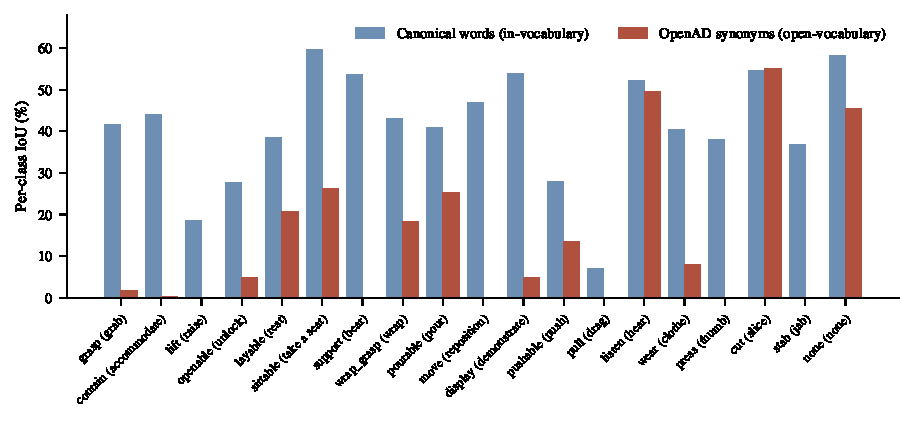
\includegraphics[width=\textwidth]{figures/fig_perclass.pdf}
\caption{Per-class IoU of the pretrained checkpoint with the canonical words and with OpenAD's synonym queries (the synonym is given in parentheses). Ten of the 18 synonyms give an IoU below 5\%, and two (slice and hear) nearly match the canonical word.}
\label{fig:perclass}
\end{figure*}

\subsection{Effect of query phrasing on the pretrained model}
Table~\ref{tab:sens} evaluates the pretrained checkpoint with the five studied affordances rephrased as held-out questions or descriptions. The mIoU changes from 41.53 with canonical words to 29.63 for questions and 30.28 for descriptions. The change is concentrated in the rephrased classes: their mean IoU goes from 48.6\% to 9.1\% (questions) and 11.9\% (descriptions), and grasp, contain and pourable drop below 0.5\% for both forms. Since the metric is a mean over 19 classes, these five classes account for $(242.8-45.3)/19=10.4$ of the 11.9 mIoU points for questions and for $(242.8-59.6)/19=9.6$ of 11.3 for descriptions (sums of the columns of Table~\ref{tab:sens}). The effect is therefore well localised, and the 14 classes that keep their canonical word account for the remaining 1.5 and 1.7 points, which probably reflect points that are reassigned to them from the rephrased classes. Cut retains a large part of its IoU (55.2\% to 43.2\% and 37.1\%), which parallels the slice example of the previous subsection and shows that the pretrained model does transfer to sentence-style queries when the geometry and the CLIP embedding of the phrase are distinctive. Plausible reasons are the distinctive geometry of the blade region and the closeness of the CLIP embeddings of the cutting phrases to that of the word ``cut''.

The score maps reveal more than the final arg-max predictions. For 40 objects, we correlated the map produced by each canonical word with those produced by its question and description. Mean Pearson correlations per affordance range from 0.60 to 0.89. The overall mean is 0.75 for canonical words versus questions and 0.74 for canonical words versus descriptions; questions and descriptions agree even more strongly, at 0.87. In other words, rephrasing often weakens the response without completely changing where the model looks. This motivated us to adapt the final mapping from point features to the text space rather than retrain the entire network. Because this analysis uses only the first 40 validation objects (22 doors and 18 clocks), we treat it as supporting rather than conclusive evidence.

\begin{table}[t]
\caption{IoU (\%) of the five studied affordances for the pretrained checkpoint, with the canonical word and with held-out question and description phrasings. The last row is the mIoU (\%) over all 19 classes. This table comes from the phrasing-sensitivity run, so its values differ slightly from Table~\ref{tab:main} (Section~\ref{sec:noise}).}
\label{tab:sens}
\centering
\small
\begin{tabular}{@{}lccc@{}}
\toprule
Affordance & Canonical & Question & Description \\
\midrule
grasp    & 42.6 & 0.0  & 0.4 \\
contain  & 43.9 & 0.0  & 0.3 \\
sittable & 59.6 & 2.0  & 21.8 \\
pourable & 41.5 & 0.0  & 0.0 \\
cut      & 55.2 & 43.2 & 37.1 \\
\midrule
Mean IoU of the five    & 48.6  & 9.1   & 11.9 \\
mIoU, 19 classes        & 41.53 & 29.63 & 30.28 \\
\bottomrule
\end{tabular}
\end{table}

\subsection{Effect of prompt-augmented fine-tuning}
Table~\ref{tab:main} and Fig.~\ref{fig:results} compare the pretrained checkpoint with the model that fine-tunes the alignment head and final feature-propagation layer. Both models were evaluated in the same run.

\emph{Held-out phrasings improve by about ten points.} On phrasings never used for training, mIoU rises from 29.27 to 40.48 for questions ($+11.21$) and from 30.40 to 40.88 for descriptions ($+10.48$). With canonical words scoring 41.28 for the pretrained model, this closes 93\% and 96\% of the gap that phrasing had opened. The change is more than twenty times the run-to-run variation of about 0.4 points (Section~\ref{sec:noise}), and it holds for phrasings that the model never saw in training. The head-only and decoder configurations reach the same level ($+10.5$ and $+10.0$, and $+10.9$ and $+10.3$; Section~\ref{sec:ablation}), so the result does not depend on a single configuration.

\emph{Seen and held-out phrasings behave alike.} Phrases from the training set improve by $+13.08$ and $+12.72$ and reach 42.12 and 42.37, the level of the canonical words (42.02). The held-out results are only 1.6 and 1.5 points below, so the network has learned a property of the phrase family and not the 35 training strings. The held-out strings differ from the training strings as wordings and not necessarily as meanings (Section~\ref{sec:conditions}), so the experiment measures generalisation across wording.

\emph{Canonical words are preserved.} The canonical mIoU changes from 41.28 to 42.02 ($+0.74$), so robustness to phrasing is gained without a cost on the original words. The checkpoint was selected for its canonical validation mIoU on the same objects (42.46 at epoch 4, Table~\ref{tab:train}), and re-evaluating it gives 42.02, so we read the result as preservation of the original performance.

\emph{Gains are largest where the pretrained model was weakest} (Fig.~\ref{fig:results}b,c). The mean IoU of the five affordances rises from 8.9\% to 43.9\% for held-out questions and from 12.1\% to 45.0\% for held-out descriptions. Averaged over the two forms, the largest gains are for sittable, contain and pourable. Grasp under the question form has the most headroom left, with an IoU of 22.2\% against about 42\% for the canonical word, while the description form reaches 40.4\%. For cut, where the pretrained model was already fairly stable, the gains are smaller ($+11$ and $+16$ points). We interpret only the larger per-class differences, since the noise of single classes has not been estimated.

\emph{Interpretation.} Only 101,377 parameters in the head and final propagation layer were updated. Section~\ref{sec:ablation} shows similar results when training either the head alone or the whole decoder. Together with the score-map correlations, this suggests that the frozen backbone already contains useful spatial information and that fine-tuning mainly improves its alignment with sentence-style queries. Directly probing the feature space would be a useful next step.

\begin{table}[t]
\caption{Pretrained versus the reported fine-tuned model (head and last propagation layer), mIoU (\%) over 19 classes, same validation objects and same query lists in one comparison run. ``Seen'' phrasings belong to the fine-tuning set, ``held-out'' phrasings do not. Bold marks the held-out conditions that define the result. All values are ours.}
\label{tab:main}
\centering
\small
\begin{tabular}{@{}lccc@{}}
\toprule
Condition & Pretrained & Fine-tuned & $\Delta$ \\
\midrule
Canonical words               & 41.28 & 42.02 & $+0.74$ \\
Question, seen                & 29.04 & 42.12 & $+13.08$ \\
\textbf{Question, held-out}   & 29.27 & \textbf{40.48} & $\mathbf{+11.21}$ \\
Description, seen             & 29.64 & 42.37 & $+12.72$ \\
\textbf{Description, held-out}& 30.40 & \textbf{40.88} & $\mathbf{+10.48}$ \\
\bottomrule
\end{tabular}
\end{table}

\begin{figure*}[t]
\centering
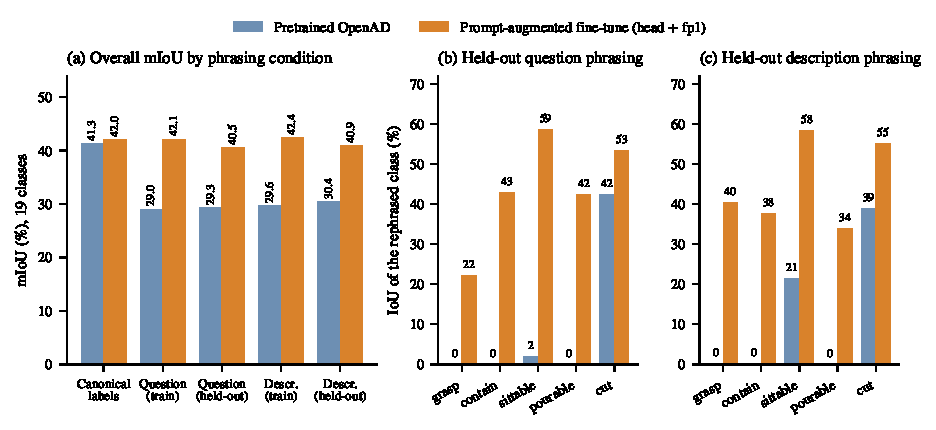
\includegraphics[width=\textwidth]{figures/fig_results.pdf}
\caption{(a) mIoU of the pretrained and the reported fine-tuned model (head and last propagation layer) under the five phrasing conditions of Table~\ref{tab:main}. (b, c) IoU of each rephrased affordance under held-out question and description phrasings. Grasp with the held-out question remains the weakest case after fine-tuning.}
\label{fig:results}
\end{figure*}

\subsection{Training behaviour}
Table~\ref{tab:train} lists the training record of the reported model. The loss falls from 0.701 to 0.639 and changes little after epoch 4. The canonical validation mIoU is 41.72 after the first epoch, at the level of the pretrained evaluations (41.25 to 41.53), reaches 42.46 at epoch 4 and stays between 41.98 and 42.23 afterwards, so the adaptation is fast and stable and preserves the original vocabulary. Epochs after the fourth are equivalent to epoch 4 within the evaluation noise. The head-only configuration behaves alike: its loss falls from 0.726 to 0.645 and its validation mIoU peaks at 42.22 at epoch 4 of 5. All three configurations of the capacity ladder select epoch 4 (Table~\ref{tab:cap}), so about four passes over the training set suffice at every capacity.

\begin{table}[t]
\caption{Fine-tuning record of the reported model (head and last propagation layer). Loss is the mean weighted NLL of the epoch. Validation mIoU uses canonical words only and is the criterion for choosing the checkpoint.}
\label{tab:train}
\centering
\small
\begin{tabular}{@{}cccc@{}}
\toprule
Epoch & Train loss & Val.\ mIoU (\%) & Time (s) \\
\midrule
1 & 0.701 & 41.72 & 880 \\
2 & 0.650 & 42.05 & 878 \\
3 & 0.645 & 42.18 & 872 \\
\textbf{4} & 0.644 & \textbf{42.46} & 856 \\
5 & 0.642 & 42.23 & 844 \\
6 & 0.641 & 41.98 & 830 \\
7 & 0.640 & 42.17 & 835 \\
8 & 0.639 & 42.15 & 839 \\
\bottomrule
\end{tabular}
\end{table}

\subsection{Ablations}
\label{sec:ablation}
The design of the conditions gives three factor comparisons, namely phrase form (question or description), exposure (seen or held-out) and model (pretrained or fine-tuned), and the capacity ladder adds a fourth factor. Form has little effect on either model (differences of 0.2 to 1.0 points in Table~\ref{tab:main}).

\emph{How much of the network to train.} The capacity ladder trains the alignment head (67,073 parameters, 5 epochs), the head together with \texttt{fp1} (101,377 parameters, 8 epochs) and the head together with the whole feature-propagation decoder (743,041 parameters, 8 epochs), with the same data, phrases, loss, learning rate and seed. The rungs differ by a factor of eleven in trainable parameters, and each is compared with the pretrained model of its own comparison run (Table~\ref{tab:ablation}). The gain is present at every rung. Head-only training already delivers $+10.5$ and $+10.0$ mIoU on held-out questions and descriptions and $+0.5$ on canonical words. Adding \texttt{fp1} raises the held-out scores by a further 0.73 and 0.61 points, to 40.48 and 40.88, the highest values of the ladder. Releasing the whole decoder gives 40.20 and 40.51, within 0.3 to 0.4 points of the previous rung and inside the range of repeated evaluations (0.41 points). The per-affordance IoUs of the head-only and head plus \texttt{fp1} models differ by less than 3 points in eight of the ten affordance and form combinations (the exceptions are grasp and cut under questions, $+7.4$ and $+4.1$ points). The ladder supports two conclusions. First, the alignment head carries nearly all of the gain, so the update that is needed is small. Second, the improvement is stable over a factor of eleven in capacity, which indicates that it is a property of the paraphrase supervision and not of a particular parameter budget. We report head plus \texttt{fp1} as the main model because it has the highest held-out scores and the highest canonical validation mIoU (Table~\ref{tab:cap}) at a small extra cost over the head alone.

\begin{table}[t]
\caption{Capacity ladder, mIoU (\%) over 19 classes. Each fine-tuned model is compared with the pretrained model of its own comparison run, so the pretrained rows differ slightly (Section~\ref{sec:noise}). The selected checkpoint is from epoch 4 in all three configurations.}
\label{tab:ablation}
\centering
\small
\begin{tabular}{@{}lcccc@{}}
\toprule
Model & Params & Canon. & Question & Descr. \\
 & trained & words & held-out & held-out \\
\midrule
Pretrained, run 1       & n/a    & 41.44 & 29.22 & 30.22 \\
Head only               & 67,073 & 41.93 & 39.75 & 40.27 \\
\quad change vs run 1   &        & $+0.49$ & $+10.53$ & $+10.04$ \\
\midrule
Pretrained, run 2       & n/a    & 41.28 & 29.27 & 30.40 \\
Head + \texttt{fp1} (reported) & 101,377 & 42.02 & 40.48 & 40.88 \\
\quad change vs run 2   &        & $+0.74$ & $+11.21$ & $+10.48$ \\
\midrule
Pretrained, run 3       & n/a    & 41.19 & 29.29 & 30.23 \\
Decoder (\texttt{fp1}--\texttt{fp3}) & 743,041 & 41.73 & 40.20 & 40.51 \\
\quad change vs run 3   &        & $+0.54$ & $+10.91$ & $+10.28$ \\
\bottomrule
\end{tabular}
\end{table}

\begin{table}[t]
\caption{Fine-tuning records of the three configurations of the capacity ladder (``Loss'' is the training loss of the last epoch). Validation mIoU uses canonical words, is the selection criterion and is the best epoch's value (epoch 4 in all three). Time is the total for all epochs, each including a full validation pass.}
\label{tab:cap}
\centering
\small
\begin{tabular}{@{}lccccc@{}}
\toprule
Config. & Params & Ep. & Loss & Val.\ (\%) & Time (s) \\
\midrule
Head only          & 67,073  & 5 & 0.645 & 42.22 & 4,261 \\
Head + \texttt{fp1}  & 101,377 & 8 & 0.639 & 42.46 & 6,834 \\
Decoder            & 743,041 & 8 & 0.656 & 42.07 & 6,726 \\
\bottomrule
\end{tabular}
\end{table}

\subsection{Open-vocabulary evaluation of the reported model}
\label{sec:ov}
Prompt-augmented fine-tuning rephrases only five affordances, so we also asked what it does to the open-vocabulary benchmark of Section~\ref{sec:repro}, in which every one of the 18 affordances is queried by a synonym. We evaluated the reported model (head and last propagation layer) with the same 18 synonym queries, the same 2,285 validation objects and the same code as the pretrained reproduction, in one evaluation pass. Table~\ref{tab:ov} gives the result. The mIoU rises from 14.40 to 18.66 ($+4.26$, more than ten times the resolution of 0.4 points of Section~\ref{sec:noise}), the point accuracy from 46.33\% to 50.20\% and the mean class accuracy from 19.63\% to 28.02\%.

\emph{The change is concentrated in the fine-tuned affordances.} Across all 19 classes, the 4.26-point mIoU increase corresponds to 80.9 total IoU points. The five studied affordances contribute 78.7 points (97\%), the 13 other affordances contribute $-0.7$, and the background class contributes $+2.9$. Mean IoU for the 13 unstudied classes changes only from 9.22\% to 9.17\%. Six of these classes (lift, support, move, pull, press, and stab) have zero IoU under both models. The remaining seven change by between $-3.1$ and $+3.5$ points (pushable $-3.1$, layable $-1.1$, openable $-0.9$, wrap $+3.5$, listen $+0.6$, display $+0.3$, and wear $0.0$). Since we have not estimated per-class noise, we do not interpret these small individual changes. The result shows no clear harm to unseen affordances, but it also provides no evidence that the improvement transfers to them.

\emph{Transfer to a new word depends on the word.} Grab for grasp (1.7\% to 36.3\%) and take a seat for sittable (26.2\% to 57.9\%) improve strongly, and slice for cut changes little (55.0\% to 56.7\%) because the pretrained model already handled it. Accommodate for contain does not transfer (0.2\% to 0.0\%), although contain improves under the held-out questions and descriptions (from below 0.3\% to 42.9\% and 37.8\% IoU). The model thus learned to answer sentence-style phrasings of contain but not this isolated synonym. We did not test why. A possible factor is that the training phrases of grasp include grip and hold, which lie close to grab, whereas those of contain (store, hold contents) may lie farther from accommodate. The semantic distance between training and test wordings is not controlled (Section~\ref{sec:conditions}).

\emph{Limits of this evaluation.} Pour is one of the fine-tuning labels of pourable, so its gain (25.2\% to 36.1\%) shows the effect of training and is not evidence of generalisation. The other four synonyms are not in the fine-tuning set and they also belong to our held-out label lists (Section~\ref{sec:conditions}). The result comes from one evaluation pass of one checkpoint, and only the reported model was evaluated on this benchmark.

\begin{table}[t]
\caption{OpenAD open-vocabulary benchmark (18 synonym queries, validation split), IoU (\%) of the pretrained checkpoint and of the reported fine-tuned model. The synonym is in parentheses. Pour is one of the fine-tuning labels of pourable, and the other four synonyms are not in the fine-tuning set. ``13 unstudied'' is the mean over the affordances that fine-tuning never rephrased. Pretrained values are those of Table~\ref{tab:repro}.}
\label{tab:ov}
\centering
\small
\begin{tabular}{@{}lccc@{}}
\toprule
 & Pretrained & Fine-tuned & $\Delta$ \\
\midrule
grasp (grab)                 & 1.7  & 36.3 & $+34.6$ \\
contain (accommodate)        & 0.2  & 0.0  & $-0.2$ \\
sittable (take a seat)       & 26.2 & 57.9 & $+31.7$ \\
pourable (pour, trained on)  & 25.2 & 36.1 & $+10.9$ \\
cut (slice)                  & 55.0 & 56.7 & $+1.7$ \\
\midrule
Mean of the 13 unstudied     & 9.22 & 9.17 & $-0.05$ \\
Background (none)            & 45.4 & 48.3 & $+2.9$ \\
\midrule
mIoU, 19 classes             & 14.40 & 18.66 & $+4.26$ \\
Point accuracy               & 46.33 & 50.20 & $+3.87$ \\
Mean class accuracy          & 19.63 & 28.02 & $+8.39$ \\
\bottomrule
\end{tabular}
\end{table}

%% ------------------------------------------------------------------
\section{Qualitative Analysis, Failure Cases and Demonstration}
\label{sec:qual}

\subsection{Examples}
Figures~\ref{fig:qualA} and~\ref{fig:qualB} show ground-truth masks and score maps for six object--affordance pairs under held-out questions. We use the reported model, which fine-tunes the alignment head and final propagation layer. For each category, we chose the first validation object whose ground truth contains the target affordance; the examples were therefore not selected by inspecting model predictions. The pairs include both common and rare categories, and all panels use the same colour scale. Each map gives the query's probability when competing only with \texttt{none}, rather than the 19-way prediction used for mIoU. The figures should therefore be read as confidence maps, not as the exact segmentations scored in Section~\ref{sec:results}. These six examples illustrate typical behaviours but do not form a statistical sample.

\emph{Clear improvement (chair, bowl).} For the chair, the pretrained model gives intermediate scores over the annotated region and its surroundings, and the fine-tuned model gives scores near 1 over most of the annotated region with a clear boundary, apart from a weaker part at its lower edge. For the bowl, the pretrained map is uniformly low to moderate, while the fine-tuned map is high on the interior surface that carries the label and moderate on the outer shell, so the region is found and its extent is slightly overestimated.

\emph{Partial improvement (knife).} Both models peak at the same small region of the blade edge, and the fine-tuned map has a stronger peak. The rest of the object receives a raised score of about 0.4 to 0.6, which agrees with the smaller aggregate gain for cut, where the pretrained model was already fairly stable.

\emph{Broad activation (mug, bottle).} For the mug, the fine-tuned map raises a near-zero pretrained response to above 0.6 over most of the object, so the object is detected as pourable while the labelled rim region is not yet delimited. For the bottle, the fine-tuned model produces a peak at the labelled patch on a background of 0.3 to 0.5, where the pretrained model produces nothing.

\emph{Failure case (bag).} For the bag, neither model gives a score above the background level on the labelled grasp region. The same affordance and question form are detected on the bottle, and the bag agrees with the lower aggregate IoU of grasp under held-out questions (22.2\% for the reported model). Plausible contributing factors are that the validation split contains only 12 bags, that the grasp region on bags (handles and body) is visually diverse, and that the sentence ``Where should I take hold of this?'' may lie far from the seven training phrases of grasp in the text space. A larger set of training phrases for grasp is a direct way to test the last factor.

Across these examples, fine-tuning raises the query score over fairly broad parts of the object. The maps are clearest when the labelled region is large, as with the chair and bowl. For smaller regions such as the mug rim, knife edge, and bottle opening, it is not yet clear whether the broader activation reduces spatial precision or simply shifts all scores upward while preserving their ranking. A threshold-free per-object measure, such as area under the ROC curve, would help distinguish these cases.

\begin{figure*}[t]
\centering
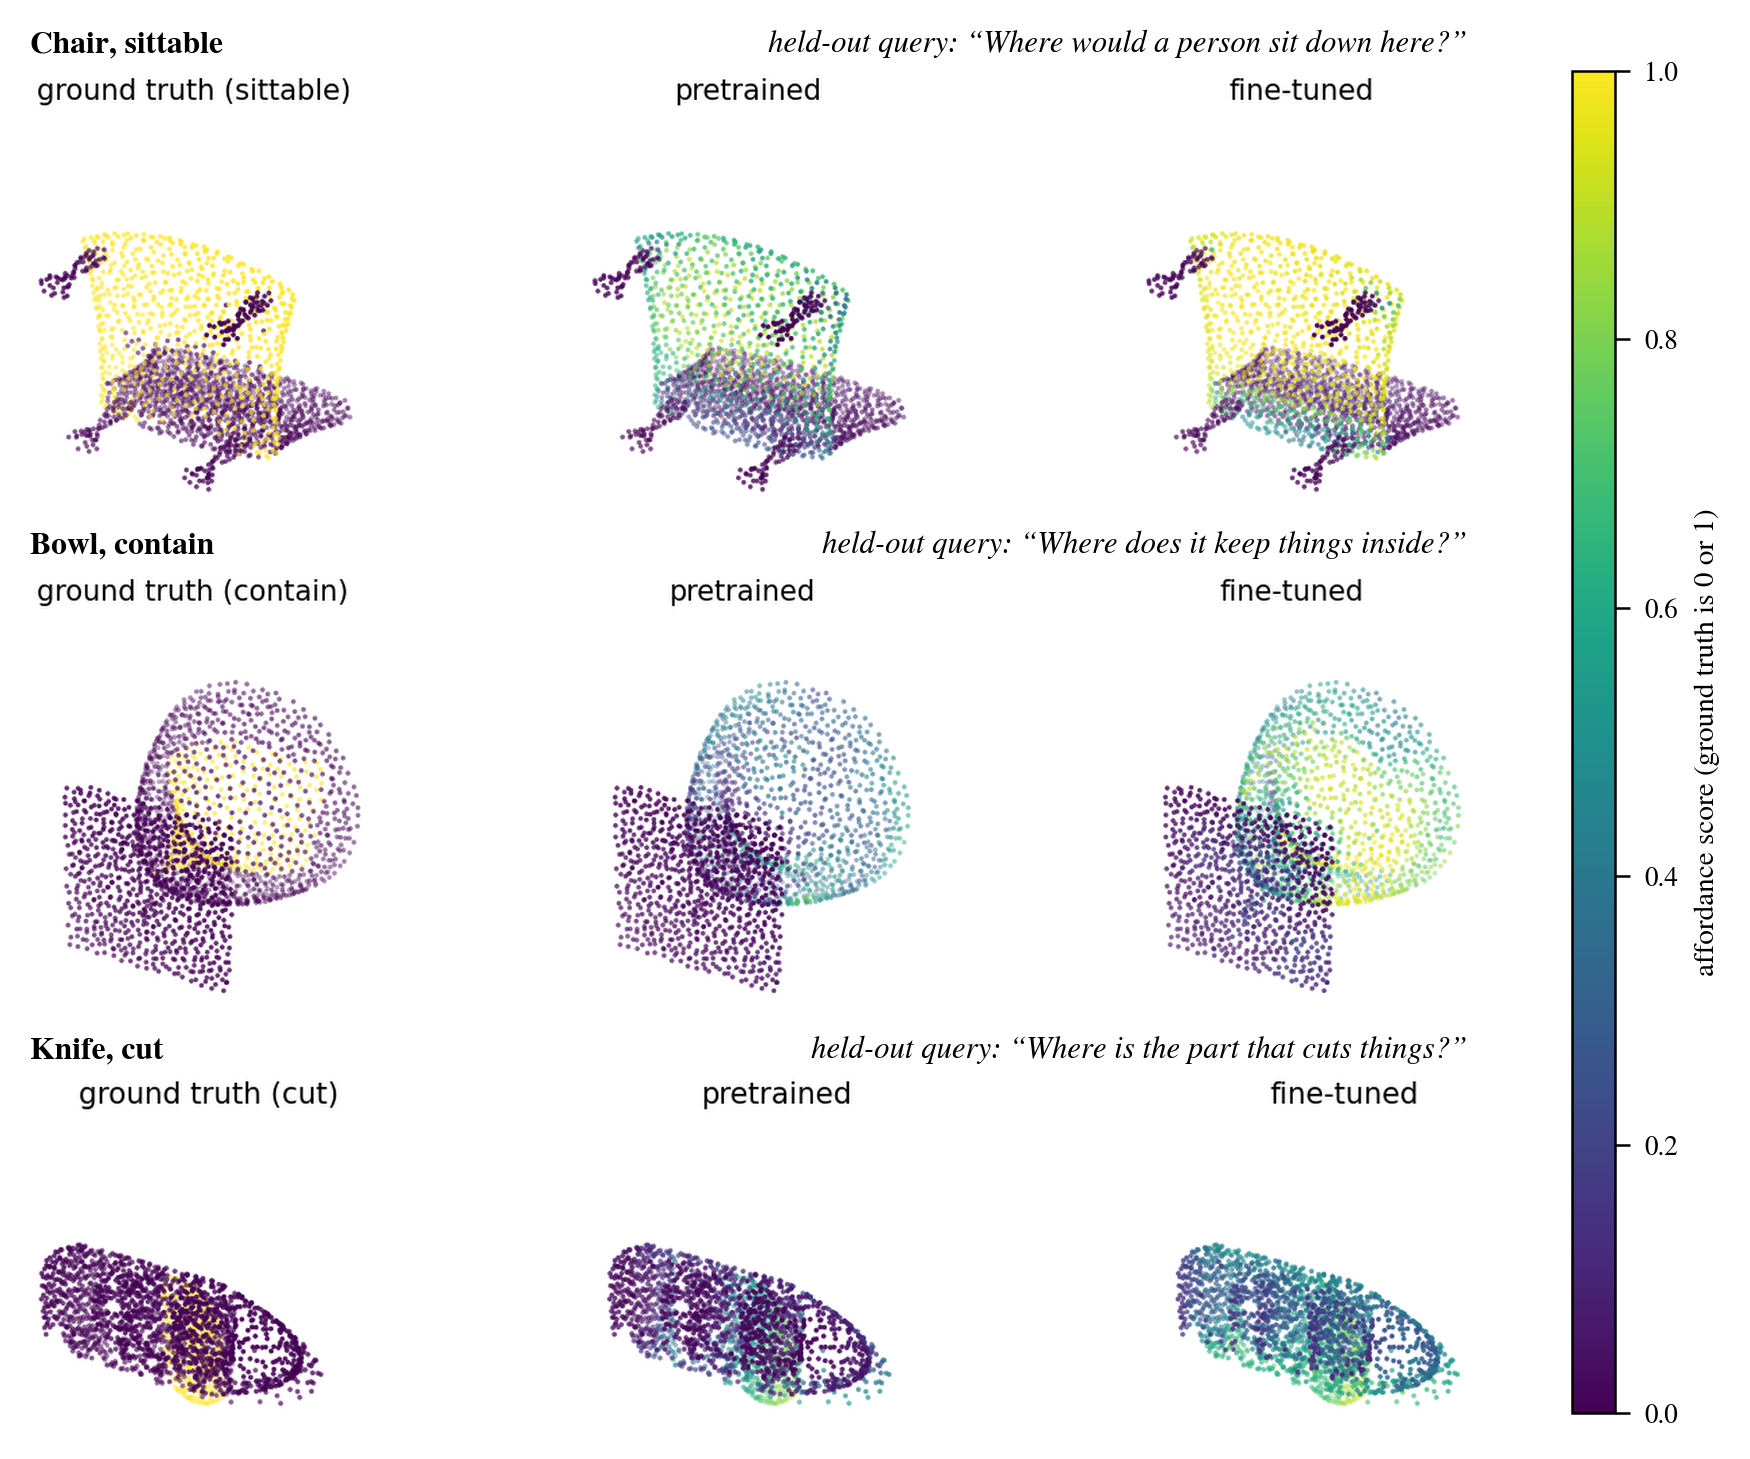
\includegraphics[width=0.76\textwidth]{figures/fig_qual_a.png}
\caption{Improvement cases with held-out question queries. From left to right the panels show the ground truth (0 or 1), pretrained score, score of the reported fine-tuned model, on the same colour scale. The fine-tuned model recovers the region for the chair and the bowl, and the knife blade shows a stronger peak with a raised background.}
\label{fig:qualA}
\end{figure*}

\begin{figure*}[t]
\centering
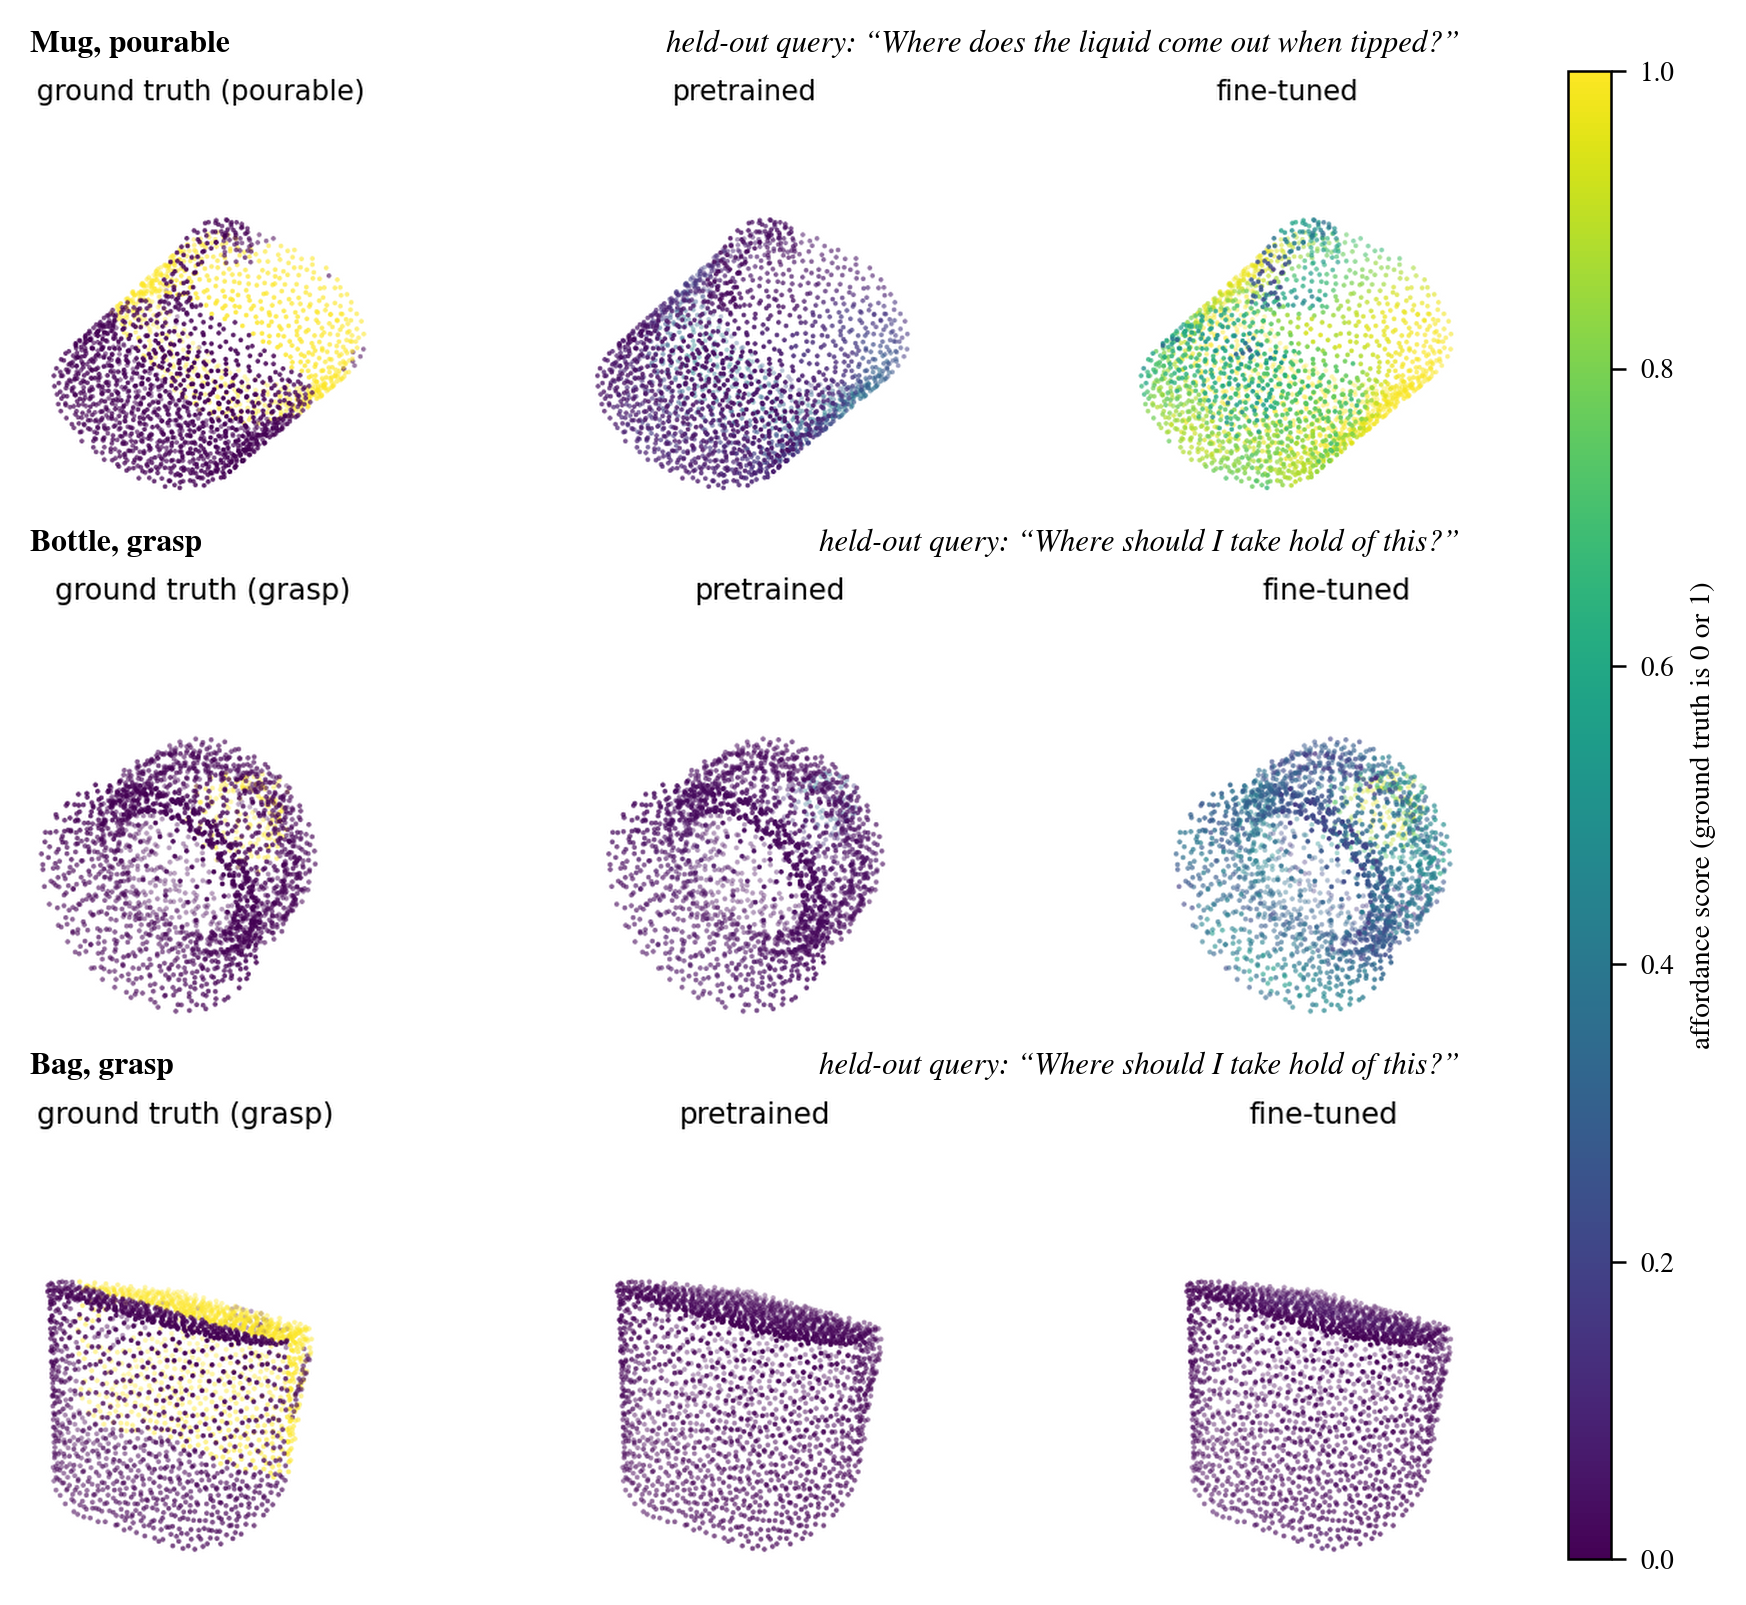
\includegraphics[width=0.76\textwidth]{figures/fig_qual_b.png}
\caption{Further cases of the reported fine-tuned model with held-out question queries. The mug shows a broad activation, the bottle a correct peak on a raised background, and the bag is a failure case of both models.}
\label{fig:qualB}
\end{figure*}

\subsection{Errors that do not depend on phrasing}
Some errors remain even with canonical wording. In Fig.~\ref{fig:perclass}, pull (7.1\%), lift (18.5\%), openable (27.7\%), and pushable (28.0\%) all have relatively low IoU. Per-object point accuracy is lowest for Bag (41\% across 12 objects), Bottle (44\% across 41), and Hat (46\% across 22), but reaches 92\% for Keyboard and 84\% for Display. These limitations belong to the underlying detector or dataset rather than to prompt phrasing, and our lightweight fine-tuning is not designed to address them.

\subsection{Interactive prototype}
The same model is exposed through an interface built with Gradio and Plotly, so that the findings above can be explored interactively. The user selects an object from the validation split and a model (pretrained or fine-tuned), types a query or picks an example, and receives a rotatable 3D point cloud coloured by the score of Eq.~\eqref{eq:align} against \texttt{none}, together with the fraction of points with a score of at least 0.5 and the peak and mean score. Predictions are cached per object, query and model, so repeated queries are immediate. The interface distinguishes four states, namely a normal result, a low-confidence result (no point reaches 0.5, flagged as unreliable), an empty query, and an inference error. It also keeps the previous query for side-by-side comparison, which lets a user see directly how the wording changes the map. These features follow from the results above: because phrasing changes the maps, comparing two wordings is useful, and because a uniformly low map can mean either an absent affordance or a phrasing failure, the interface states its uncertainty explicitly. The logic of the backend is unit tested. Usability is examined in a separate report on the human-computer interaction aspects of the project.

%% ------------------------------------------------------------------
\section{Scope and Extensions}
\label{sec:limits}

\textbf{Statistics.} Each reported number comes from one evaluation pass and one fine-tuning run per configuration, all using seed 1. Repeated evaluation suggests a variation of about 0.4 mIoU (Section~\ref{sec:noise}), so we avoid drawing conclusions from smaller total differences or modest per-class changes. The similar gains across all three training configurations provide some evidence that the main effect is stable, but experiments with additional seeds are still needed.

\textbf{Data.} The distributed data contain a training and a validation split and no separate test split. The validation split serves to choose the epoch, by the canonical mIoU alone, and for the final evaluation. Held-out phrasings play no role in the choice of the epoch. The choice of the reported configuration among the three rungs of the ladder used the held-out scores, and all three rungs are therefore reported.

\textbf{Phrasing.} We study five of the 18 affordances, with one held-out question and one held-out description for each. This gives a controlled test of new wording, but ten strings cannot represent the full range of language users may produce. The held-out strings do not overlap with training strings, although we do not control their semantic similarity. The same protocol could be extended with larger and more varied phrase sets.

\textbf{Interpretation.} The score-map analysis used 40 objects, all doors or clocks, and gives indicative evidence. The account of why phrasing matters (Section~\ref{sec:method}) and why a small update suffices follows from aggregate metrics, and an analysis of the embedding space is a natural extension.

\textbf{Extensions.} The protocol extends directly to a canonical-only fine-tuning control (the \texttt{--no-augment} option of our script), to the open-vocabulary (synonym) evaluation of the other two rungs of the capacity ladder, which we ran only for the reported model (Section~\ref{sec:ov}), to fine-tuning of the full network including the encoder, and to further seeds. These are the first of the next steps listed in Section~\ref{sec:conclusion}.

%% ------------------------------------------------------------------
\section{Conclusion}
\label{sec:conclusion}

We reproduced OpenAD's open-vocabulary result with the released checkpoint, obtaining 14.40 mIoU compared with the published 14.37. Using the same evaluation pipeline, we found that replacing five canonical labels with natural questions or descriptions lowers mIoU by roughly 12 points. The score maps remain spatially related across wordings, but the rephrased classes often lose against classes that retain their original labels.

Prompt-augmented fine-tuning largely corrects this weakness. Updating 101,377 parameters in the alignment head and final propagation layer recovers 93\% of the lost performance for held-out questions and 96\% for held-out descriptions, while preserving performance on canonical words. Training only the head gives nearly the same improvement, and expanding the update to the whole decoder adds little. On OpenAD's synonym benchmark, mIoU rises from 14.40 to 18.66, with 97\% of the improvement coming from the five affordances included in fine-tuning. The remaining classes are essentially unchanged.

These results suggest that OpenAD already retains much of the necessary spatial information but needs better exposure to the ways people express an affordance. The current evidence is limited to five affordances, ten held-out phrases, and one training seed. Future work should include more varied prompts, additional seeds, a canonical-only fine-tuning control, synonym evaluation at every unfreezing depth, and objectives that directly encourage consistent maps across paraphrases.

\textbf{Availability.} Code, frozen prompt sets and the commands that produce every table are in the repository cited in the introduction. The figures of this report are generated from the stored metric files by a script in the same repository. The data and the pretrained checkpoint are those released by the OpenAD authors and are not redistributed. OpenAD is released under the MIT licence.

\begin{thebibliography}{00}
\bibitem{gibson1979} J. J. Gibson, \emph{The Ecological Approach to Visual Perception}. Boston, MA, USA: Houghton Mifflin, 1979.
\bibitem{affordancenet} S. Deng, X. Xu, C. Wu, K. Chen, and K. Jia, ``3D AffordanceNet: A benchmark for visual object affordance understanding,'' in \emph{Proc. IEEE/CVF Conf. Computer Vision and Pattern Recognition (CVPR)}, 2021.
\bibitem{openad} T. Nguyen, M. N. Vu, A. Vuong, D. Nguyen, T. Vo, N. Le, and A. Nguyen, ``Open-vocabulary affordance detection in 3D point clouds,'' in \emph{Proc. IEEE/RSJ Int. Conf. Intelligent Robots and Systems (IROS)}, 2023, arXiv:2303.02401.
\bibitem{clip} A. Radford, J. W. Kim, C. Hallacy, A. Ramesh, G. Goh, S. Agarwal, G. Sastry, A. Askell, P. Mishkin, J. Clark, G. Krueger, and I. Sutskever, ``Learning transferable visual models from natural language supervision,'' in \emph{Proc. Int. Conf. Machine Learning (ICML)}, 2021.
\bibitem{o2oafford} K. Mo, Y. Qin, F. Xiang, H. Su, and L. Guibas, ``O2O-Afford: Annotation-free large-scale object-object affordance learning,'' in \emph{Proc. Conf. Robot Learning (CoRL)}, 2022.
\bibitem{iagnet} Y. Yang, W. Zhai, H. Luo, Y. Cao, J. Luo, and Z.-J. Zha, ``Grounding 3D object affordance from 2D interactions in images,'' in \emph{Proc. IEEE/CVF Int. Conf. Computer Vision (ICCV)}, 2023.
\bibitem{laso} Y. Li, N. Zhao, J. Xiao, C. Feng, X. Wang, and T.-S. Chua, ``LASO: Language-guided affordance segmentation on 3D object,'' in \emph{Proc. IEEE/CVF Conf. Computer Vision and Pattern Recognition (CVPR)}, 2024.
\bibitem{vo2024} T. V. Vo, M. N. Vu, B. Huang, T. Nguyen, N. Le, T. Vo, and A. Nguyen, ``Open-vocabulary affordance detection using knowledge distillation and text-point correlation,'' in \emph{Proc. IEEE Int. Conf. Robotics and Automation (ICRA)}, 2024.
\bibitem{pointclip} R. Zhang, Z. Guo, W. Zhang, K. Li, X. Miao, B. Cui, Y. Qiao, P. Gao, and H. Li, ``PointCLIP: Point cloud understanding by CLIP,'' in \emph{Proc. IEEE/CVF Conf. Computer Vision and Pattern Recognition (CVPR)}, 2022.
\bibitem{openscene} S. Peng, K. Genova, C. Jiang, A. Tagliasacchi, M. Pollefeys, and T. Funkhouser, ``OpenScene: 3D scene understanding with open vocabularies,'' in \emph{Proc. IEEE/CVF Conf. Computer Vision and Pattern Recognition (CVPR)}, 2023.
\bibitem{pointnet} C. R. Qi, H. Su, K. Mo, and L. J. Guibas, ``PointNet: Deep learning on point sets for 3D classification and segmentation,'' in \emph{Proc. IEEE Conf. Computer Vision and Pattern Recognition (CVPR)}, 2017.
\bibitem{pointnet2} C. R. Qi, L. Yi, H. Su, and L. J. Guibas, ``PointNet++: Deep hierarchical feature learning on point sets in a metric space,'' in \emph{Advances in Neural Information Processing Systems (NeurIPS)}, 2017.
\bibitem{dgcnn} Y. Wang, Y. Sun, Z. Liu, S. E. Sarma, M. M. Bronstein, and J. M. Solomon, ``Dynamic graph CNN for learning on point clouds,'' \emph{ACM Trans. Graphics}, vol. 38, no. 5, 2019.
\bibitem{coop} K. Zhou, J. Yang, C. C. Loy, and Z. Liu, ``Learning to prompt for vision-language models,'' \emph{Int. J. Computer Vision}, vol. 130, no. 9, 2022.
\bibitem{kumar2022} A. Kumar, A. Raghunathan, R. Jones, T. Ma, and P. Liang, ``Fine-tuning can distort pretrained features and underperform out-of-distribution,'' in \emph{Proc. Int. Conf. Learning Representations (ICLR)}, 2022.
\bibitem{clipadapter} P. Gao, S. Geng, R. Zhang, T. Ma, R. Fang, Y. Zhang, H. Li, and Y. Qiao, ``CLIP-Adapter: Better vision-language models with feature adapters,'' \emph{Int. J. Computer Vision}, vol. 132, 2024.
\bibitem{wortsman2022} M. Wortsman, G. Ilharco, J. W. Kim, M. Li, S. Kornblith, R. Roelofs, R. Gontijo-Lopes, H. Hajishirzi, A. Farhadi, H. Namkoong, and L. Schmidt, ``Robust fine-tuning of zero-shot models,'' in \emph{Proc. IEEE/CVF Conf. Computer Vision and Pattern Recognition (CVPR)}, 2022.
\bibitem{adam} D. P. Kingma and J. Ba, ``Adam: A method for stochastic optimization,'' in \emph{Proc. Int. Conf. Learning Representations (ICLR)}, 2015.
\bibitem{batchnorm} S. Ioffe and C. Szegedy, ``Batch normalization: Accelerating deep network training by reducing internal covariate shift,'' in \emph{Proc. Int. Conf. Machine Learning (ICML)}, 2015.
\end{thebibliography}

\end{document}
